%%%%%%%%%%%%%%%%%%%%%%%%%%%%%%%%%%%%%%%%%%%%%%%%%%%%%%%%%%%%%%%%%%%%%%%%%%%%%%%%%%%%%%%%%%%%%%%%%%%
%%%%%%%%%%%%%%%%%%%%%%%%%%%%%%%%%%%%%%%%%%%%%%%%%%%%%%%%%%%%%%%%%%%%%%%%%%%%%%%%%%%%%%%%%%%%%%%%%%%
%%%%%%%%%%%%%%%%%%%%%%%%%%%%%%%%%%%%%%%%%%%%%%%%%%%%%%%%%%%%%%%%%%%%%%%%%%%%%%%%%%%%%%%%%%%%%%%%%%%
%%%%%%%%%%%%%%%%%%%%%%%%%%%%%%%%%%%%%%%%%%%%%%%%%%%%%%%%%%%%%%%%%%%%%%%%%%%%%%%%%%%%%%%%%%%%%%%%%%%

\section{Matemáticas}

%
%El cuerpo central de este trabajo es averiguar sin este modelo de tipo estocástico para los datos
%permite la hipótesis de que los procesos estocásticos involucrados son estacionarios, cuando menos en
%un sentido débil.

Existe una larga tradición en las ciencias biomédicas para entender (y modelar) las señales
electrofisiológicas en términos de ondas y frecuencias, en parte debido a que fundamentalmente son
fenómenos eléctricos \cite{Kaiser00}.
El enfoque que se aborda, a \textit{grosso modo}, es asociar la \textit{energía} de una señal con 
la norma inducida por un producto interno, luego usar una base de un espacio (\textit{componentes 
de frecuencia}) para estudiar cómo se reparte esta energía entre tales elementos;
en concreto,
esto se logrará usando una generalización de la base Fourier para la familia de 
procesos estocásticos \textit{semi-estacionarios}.

Cabe mencionar que se propone como hipótesis que las señales constituyen un fenómeno 
predominantemente estocástico; esto no significa que las señales sean completamente aleatorias, sino 
que el posible no-determinismo está considerado en el modelo.
Por otro lado, aunque las señales sólo son registrables en un conjunto finito de puntos en el 
tiempo, se supone que el fenómeno ocurre efectivamente \textit{a tiempo continuo}, lo cual 
permitirá asumir algunas propiedades para el modelo.

Una vez formulado el modelo descrito, el objetivo principal es estudiar si éste es adecuado (en un 
sentido estadístico) para las señales que conforman el polisomnograma, o si pueden se explicadas
mejor como procesos estocásticos déblimente estacionarios (un modelo más particular). Dado el 
enfoque descrito, la comparación entre modelos se hará \textit{en términos ondas y frecuencias}.

%%%%%%%%%%%%%%%%%%%%%%%%%%%%%%%%%%%%%%%%%%%%%%%%%%%%%%%%%%%%%%%%%%%%%%%%%%%%%%%%%%%%%%%%%%%%%%%%%%%

\subsection{Transformada de Fourier}

%Un concepto base para estudiar la distribución de energía en componentes de frecuencia, en el
%sentido clásico, es el de la

La exposición inicia con los espacios de las \textbf{series $\boldsymbol{p}$-sumables}
($\lp$), y las  \textbf{funciones $\boldsymbol{p}$-integrables} sobre un intervalo 
$I \subseteq \R$ ($\llp$).
%; en el presente trabajo sólo se usarán los casos $p=1,2$.
%
%\begin{align}
%\ell^{p} &:= \left\{ s: \Z\rightarrow\C \talque \sum_{n=-\infty}^{\infty} \abso{s(n)}^{p} < \infty \right\}
%\label{lpdef} \\
%L^{p}[I] &:= \left\{ S: I\rightarrow\C \talque \int_I \abso{S(t)}^{p} dt < \infty \right\}
%\label{llpdef}
%\end{align}
\begin{align*}
\ell^{p} &:= \left\{ s: \Z\rightarrow\C \talque \sum_{n=-\infty}^{\infty} \abso{s(n)}^{p} < \infty \right\}
\\
L^{p}[I] &:= \left\{ S: I\rightarrow\C \talque \int_I \abso{S(t)}^{p} dt < \infty \right\}
\end{align*}

Estos espacios admiten las operaciones $+$, $\cdot$ y multiplicación por escalares complejos de la 
manera usual.%, es decir

%\begin{align*}
%s, z \in \lp, c \in \C \Rightarrow 
%[s+z](n) &= s(n) + z(n) \\
%[s\cdot z](n) &= s(n) z(n) \\
%[c \cdot s](n) &= s(n)c \\
%S, Z \in \llp, c \in \C \Rightarrow 
%[S+Z](t) &= S(t) + Z(t) \\
%[S\cdot Z](t) &= S(t)  Z(t) \\
%[c \cdot S](t) &= S(t)c
%\end{align*}
%
%En las próximas líneas se seguirán usando $s, z, S, Z, c$.

Para el caso particular $p=2$, los conjuntos $\ldos$ y $\lldos$ admiten los siguientes productos 
internos:
%
\begin{align*}
\left\langle s,z \right\rangle &= \sum_{n=-\infty}^{\infty} s(n) \overline{z(n)}\\
\left\langle S,Z \right\rangle &= \int_I S(t) \overline{Z(t)} dt
\end{align*}

Usando dichos productos internos, junto con las normas y métricas que inducen, los conjuntos 
$\ldos$ y $\lldos$ tienen estructura de \textbf{espacio de Hilbert}.

Con las definiciones anteriores, que muestran que $\ldos$ y $\lldos$ son \textit{muy}
parecidos, se puede formular unaa definición para la transformada de Fourier como una equivalencia
entre estos espacios.

%{De manera pragm\'atica, en el presente trabajo la 
%palabra  'frecuencia' se usar\'a para referirse a la cantidad $q$ en expresiones del tipo 
%$e^{i q t}$}

\begin{definicion}[Serie de Fourier]
Sea $S: \R \rightarrow \C$ una función periódica con periodo $2T$ y tal que 
$S \in L^{2}\left[[-T,T]\right]$. Se dice que $A$ es la serie de Fourier para $S$ si cumple que
\begin{equation*}
A(n) = \frac{1}{2 T} \simint{T} S(t) e^{-\nicefrac{ i \abso{n} t}{2T}} dt
\end{equation*}
%Adicionalmente, la función $\mathcal{F} : \lldos \rightarrow \ldos : S \mapsto A$  recibe el nombre
%de \textbf{Transformada de Fourier}
\label{FourierClasico}
\end{definicion}

\begin{definicion}[Transformada de Fourier]
Sean $S$ y $A$ como en la definción \ref{FourierClasico}. Se le llama transformada de Fourier a la
función $\mathcal{F}_T : L^{2}\left[[-T,T]\right] \rightarrow \ldos : S \mapsto A$
\end{definicion}

Puede interpretarse a $A$ como las coordenadas de $S$ en $L^{2}\left[[-T,T]\right]$, usando la base 
ortonormal $\left\{ e^{\nicefrac{i \abso{n} t}{2 T}} \right\}_{n\in \Z}$ que es conocida
como la \textbf{base de Fourier}.
Se demuestra en el anexo () que $\mathcal{F}$ está bien definida en el sentido de 
tener efectivamente el dominio y codominio indcados. Así mismo, son demostradas las siguientes
propiedades:
\begin{itemize}
\item $\mathcal{F}$ es lineal, es decir, $\mathcal{F}[cS + Z] = c\mathcal{F}[S] + \mathcal{F}[Z]$

\item $\mathcal{F}$ \textbf{no} es invertible, aunque se suele definir una pseudoinversa
\begin{equation*}
\mathcal{F}_{T}^{\text{inv}} : \ldos \rightarrow L^{2}\left[[-T,T]\right] :
A \mapsto \sum_{n -\infty}^{\infty} A(n) e^{\nicefrac{i \abso{n} t}{2 T}}
\end{equation*}
\end{itemize}

Con esta terminología se define, de manera pragmática, la \textbf{energía disipada} y la 
\textbf{potencia} de una función $S$ en un intervalo $[a,b]$ como 
\begin{align*}
\text{energía}[S]_{[a,b]} &= \int_a^{b} \abso{S(t)}^{2} dt \\
\text{potencia}[S]_{[a,b]} &= \frac{1}{b-a} \int_a^{b} \abso{S(t)}^{2} dt
\end{align*}
%
%Estas últimas definiciones cobran importancia a la luz del teorema \ref{parseval}: la energía de 
%una función equivale a su norma.

Una conseceuncia interesante de este concepto de energía frente al teorema \ref{parseval} es que la 
energía disipada por una función equivale a la suma de la energía disipada por sus 
\textit{componentes} en la base de Fourier.
Conviene, entonces, definir una función que \textit{desglose} estos \textit{aportes}.

\begin{teorema}[Parseval]
Sea $S \in L^{2}\left[[-T,T]\right]$, y sea $A = \mathcal{F}[S]$. Se cumple que
\begin{equation*}
\int_{-T}^{T} \abso{S(t)}^{2} dt = \sum_{n=-\infty}^{\infty} \abso{A(n)}^{2}
\end{equation*}
\label{parseval}
\end{teorema}

\begin{definicion}[Espectro de potencias]
Sea $S \in L^{2}\left[[-T,T]\right]$, y sea $A = \mathcal{F}[S]$. Se llama espectro de potencias 
para $S$ a la función $h_S : \R \rightarrow \R $, definida como
\begin{equation*}
h_S(\omega) = 
\begin{cases}
\abso{A(n)}^{2} & \text{ , si } \omega = \nicefrac{n}{2T}, \text{   con } n\in \mathbb{Z} \\
0 & \text{ ,  otro caso}
\end{cases}
\end{equation*}
\label{espec}
\end{definicion}

Antes de pasar de tema, conviene introducir en estos espacios una tercera operación binaria llamada 
\textbf{convolución}, $\ast$, definida como
%
\begin{align*}
[s \ast z] (\tau) &= \sum_{n=-\infty}^{\infty} s(n) \overline{z(\tau-n)} \\
[S \ast Z] (\tau) &= \int_I S(t) \overline{Z(\tau-t)}
\end{align*}
%
donde $\overline{c}$ es el conjugado complejo de $c$. La convolución es conmutativa y asociativa
con la suma. Una motivación para ello es el siguiente teorema
%
\begin{teorema}%[de la convolución]
Sean $S,Z \in L^{2}\left[[-T,T]\right]$, entonces se satisface que
\begin{align*}
\mathcal{F}_T[S\ast Z]  &= \mathcal{F}_T[S] \cdot \mathcal{F}_T[Z] \\
\mathcal{F}_T[S\cdot Z] &= \mathcal{F}_T[S] \ast  \mathcal{F}_T[Z] \\
\end{align*}
\end{teorema}

%%%%%%%%%%%%%%%%%%%%%%%%%%%%%%%%%%%%%%%%%%%%%%%%%%%%%%%%%%%%%%%%%%%%%%%%%%%%%%%%%%%%%%%%%%%%%%%%%%%

\subsection{Estacionariedad débil}

\begin{definicion}[Proceso estoc\'astico]
Un proceso estoc\'astico \xt es una familia de variables aleatorias reales, 
indexadas por $t \in T$.
\label{proc_estocastico}
\end{definicion}

Respecto al conjunto $T$ que indexa a un proceso estoc\'astico, y que ser\'a referido como 
\textit{tiempo}, conviene introducir dos grandes grupos para los mismos
\begin{itemize}
\item \textit{Continuo} si $T$ es un intervalo cerrado
\item \textit{Discreto} si $T$ es de la forma 
$\{ t_0 + n \delta \lvert n \in U \subseteq \mathbb{Z} \}$
\end{itemize}

Los procesos a tiempo discreto contemplan conjuntos finitos e infinitos de puntos en el tiempo.
No se manejan discutir\'a sobre otros tipos de tiempo en este trabajo.

Como notaci\'on, se usar\'a \xt  para el proceso estoc\'astico y $X(t)$ para una de las variables
aleatorias que lo componen; de la misma manera $x(t)$ es una realizaci\'on de $X(t)$ y $F_{X(t)}$ 
es la funci\'on de probabilidad acumulada para $X(t)$.

\begin{definicion}[Estacionariedad d\'ebil]
Un proceso estoc\'astico \xt es d\'ebilmente estacionario si y s\'olo si para cualesquiera tiempos 
admisibles\footnote{El t\'ermino \textit{tiempos admisibles} significa que la definición es la misma
para diferentes tipos de tiempo, bajo las restricciones pertinente} $t$, $s$ se tiene que
\begin{itemize}
\item $\E{X(t)} = \mu_X$
\item $\Var{X(t)} = \sigma^{2}_X$
\item $\Cov{X(t),X(s)} = \rho_X (s-t)$
\end{itemize}
Donde $\mu_X$, $\sigma^{2}_X$ son constantes, $\rho_X(\tau)$ es una funci\'on que \'unicamente 
depende de $\tau$
\label{est_orden_primera}
\end{definicion}

Adicionalmente se supondrá que las señales en el electroencefalograma (EEG) son continuas, cuando menos
el sentido de media cuadrática

\begin{definicion}[Continuidad estoc\'astica en media cuadr\'atica]
Un proceso estoc\'astico a tiempo continuo $\{ X(t) \}$ es estoc\'asticamente continuo, en el 
sentido de media cuadr\'atica, en un tiempo admisible $t_0$ si y s\'olo si
\begin{equation*}
\lim_{t \rightarrow t_0} \E{\left( X(t) - X(t_0) \right)^{2}} = 0
\end{equation*}
\label{cont_est}
\end{definicion}

\subsubsection{Función de densidad espectral}

\begin{definicion}[Funci\'on de densidad espectral (FDE)]
Sea $\{X(t)\}$ un proceso estoc\'astico en tiempo continuo, d\'ebilmente estacionario. Se define la 
funci\'on de densidad espectral (FDE) para $\{X(t)\}$ como
%\begin{equation*}
%h(\omega) = \lim_{T\rightarrow \infty} \E{ \frac{ \left| G_T(\omega) \right|^{2}}{2 T} }
%\end{equation*}
\begin{equation*}
h(\omega) = \lim_{T\rightarrow \infty} \E{ \frac{1}{2T} \frac{1}{2 \pi}
\abso{ \int_{-T}^{T} X(t) e^{-i \omega t} dt}^{2} }
\end{equation*}
%Donde $G_T (\omega) = \frac{1}{\sqrt{2 \pi}} \int_{-T}^{T} X(t) e^{-i \omega t} dt$
\label{FDE}
\end{definicion}

\begin{definicion}[Funci\'on de espectro integrado]
Sea $\{X(t)\}$ un proceso estoc\'astico a tiempo continuo, d\'ebilmente estacionario. Se define la 
funci\'on de espectro integrado para $\{X(t)\}$ como
\begin{equation*}
H(\omega) = \int_{-\infty}^{\omega} h(\lambda) d\lambda
\end{equation*}
Donde $h$ es la funci\'on de densidad espectral para $\{X(t)\}$
\label{FDE_integrado}
\end{definicion}

Si la FDE, $h$, est\'a bien definida en todos sus puntos, entonces la funci\'on de espectro 
integrado ($H$) satisface que $H\prima= h$ y se dir\'a que el proceso tiene un \textbf{espectro 
puramente continuo}; si $H$ tiene una forma escalonada, con escalones rectos, se dir\'a que es un 
\textbf{espectro puramente discreto}.
Como es de esperarse, cada tipo de proceso tiene caracter\'istica diferentes y se puede estudiar 
mejor con herramientas diferentes; para el caso de procesos con un espectro mixto (ninguno de los 
anteriores), se exhiben herramientas que los reducen a estos casos 'puros'.

Cabe destacar que, por como se defini\'o la FDE integrada, \'esta es una funci\'on positiva, 
no-decreciente, y que en $-\infty$ vale 0; esta observaci\'on ser\'a importante.

\begin{teorema}[Wiener-Khinchin]
Una condici\'on suficiente y necesaria para que $\rho$ sea una funci\'on de autocorrelaci\'on de 
alg\'un proceso estoc\'astico a tiempo continuo $\{X(t)\}$ d\'ebilmente estacionario y 
estoc\'asticamente continuo, es que exista una funci\'on $F$ que tenga las siguientes propiedades
\begin{itemize}
\item Mon\'otonamente creciente
\item $F(-\infty) = 0$
\item $F(+\infty) = 1$
\end{itemize}
y tal que para todo $\tau \in \R$ se cumple que
\begin{equation*}
\rho(\tau) = \intR e^{i \omega \tau} dF(\omega)
\end{equation*}
\label{t_wienerkhinchin}
\end{teorema}

\begin{teorema}[Wold]
Una condici\'on suficiente y necesaria para que $\rho$ sea una funci\'on de autocorrelaci\'on de 
alg\'un proceso estoc\'astico a tiempo discreto $\{X(t)\}$ d\'ebilmente estacionario es que exista 
una funci\'on $F$ con las siguientes propiedades
\begin{itemize}
\item Mon\'otonamente creciente
\item $F(-\pi) = 0$
\item $F(+\pi) = 1$
\end{itemize}
y tal que para todo $\tau \in \R$ se cumple que
\begin{equation*}
\rho(\tau) = \intPI e^{i \omega \tau} dF(\omega)
\end{equation*}
\label{t_wold}
\end{teorema}

\subsection{Representación espectral}

\begin{teorema}
Sea $\{X(t)\}$ un proceso estoc\'astico a tiempo continuo d\'ebilmente estacionario de media 0 y 
estoc\'asticamente continuo en el sentido de media cuadr\'atica. Entonces, existe un proceso 
ortogonal $\{Z(\omega)\}$ tal que, para todo tiempo $\omega$ admisible, se puede 
escribir\footnote{La integral se encuentra definida en el sentido de media cuadr\'atica.}
\begin{equation*}
X(t) = \intR e^{i t \omega} dZ(\omega)
\end{equation*}
Donde el proceso $\{Z(t)\}$ tiene las siguientes propiedades para todo $\omega$
\begin{itemize}
\item $\E{dZ(\omega)} = 0$
\item $\E{\abso{dZ(\omega)}^{2}} = dH(\omega)$
\item $\Cov{dZ(\omega),dZ(\lambda)} = 0 \Leftrightarrow \omega \neq \lambda$
\end{itemize}
Donde $dH(\omega)$ la FDE integrada de $\{X(t)\}$
\label{rep_espectral}
\end{teorema}

En virtud del teorema de Wold, se puede tener una variante del teorema \ref{rep_espectral}
para procesos a tiempo discreto, raz\'on por la cual  
tal representaci\'on es referida como \textbf{representaci\'on de Wold-Cram\'er}.

%%%%%%%%%%%%%%%%%%%%%%%%%%%%%%%%%%%%%%%%%%%%%%%%%%%%%%%%%%%%%%%%%%%%%%%%%%%%%%%%%%%%%%%%%%%%%%%%%%%

\subsection{Estimóacin}

Conviene introducir estimadores para la funci\'on de autocovarianza de un proceso d\'ebilmente 
estacionario, $\{ X(t) \}$, a partir de un conjunto de $N$ observaciones equiespaciadas en el 
tiempo con separaci\'on $\Delta t$; se denotar\'a a estas observaciones como 
$x_1, x_2 , \dots, x_N$. Como se cumple la siguiente propiedad para la funci\'on de autocovarianza, 
$R$, por definici\'on
\begin{equation*}
R(\tau) = \E{X(n\Delta t)X(n\Delta t + \tau)} \text{  ,  } n = 0, 1, 2,  3,\dots, N
\end{equation*}
el estimados est\'andar para $R$ est\'a dado por la siguiente expresi\'on
\begin{equation*}
\widehat{R}(\tau) = \frac{1}{N-\abso{\tau}} 
\sum_{t = 1}^{N-\abso{\tau}} x_t x_{t+\abso{\tau}}
\label{estimador_R}
\end{equation*}

Se puede demostrar que $\widehat{R}$ es un estimador insesgado\footnote{Un estimador para el 
par\'ametro $\theta$, $\widehat{\theta}$, se dice \textbf{insesgado} si 
$\E{\widehat{\theta}}=\theta$} y consistente\footnote{Un estimador para el par\'ametro $\theta$ que 
depende de $N$ observaciones, 
$\widehat{\theta}_N$, se dice \textbf{consistente} si 
$\lim_{N\rightarrow \infty} \Var{\widehat{\theta}_N} = 0$} 
para $R$; sin embargo conviene introducir un estimador diferente para $R$
\begin{equation*}
\aste{R}(\tau) = \frac{1}{N} 
\sum_{t = 1}^{N-\abso{\tau}} x_t x_{t+\abso{\tau}}
\label{estimador_R_ast}
\end{equation*}

\begin{teorema}
Sean $x_1, x_2 , \dots, x_N$ observaciones de un proceso estoc\'astico de media cero y varianza
finita. Se puede calcular el periodograma para estos datos como
\begin{equation*}
I_N(\omega) = 2 \sum_{r = -(N-1)}^{N-1} \aste{R}(r) \COS{r \omega}
\end{equation*}
Donde $\aste{R}$ es el estimador para la funci\'on de autocovarianza del proceso, calculado como
$\widehat{R}(\tau) = \frac{1}{N-\abso{\tau}} \sum_{t = 1}^{N-\abso{\tau}} x_t x_{t+\abso{\tau}}$
\label{periodograma_rho}
\end{teorema}

Se puede demostrar que el periodograma es un estimador insesgado de la FDE para los proceso 
considerados; sin embargo, si el proceso tuviera un espectro puramente continuo, ocurre que 
$\lim_{N\rightarrow \infty} \Var{I_N(\omega)} = h^{2}(\omega)$, con $h$ la FDE del proceso: el 
periodograma, en general, no es consistente.
En parte esto ocurre porque el periodograma depende de los estimadores para la funci\'on de 
autocovarianza, $\est{R}$, evaluada en todos los puntos posibles: para calcular $\est{R}$ en 
valores muy altos se requieren puntos muy alejados, los cuales son menos abundantes e implican 
una mayor varianza.

Si efectivamente el periodograma aumenta su varianza cuando incluye las 'colas' de la funci\'on de 
autocovarianza, entonces una soluci\'on es evitarlas, multiplicando por una funci\'on de pesos. 
Tales consideraciones dan origen a estimadores de la forma
\begin{equation*}
\est{h}(\omega) = \frac{1}{2\pi} \sum_{s = -(N-1)}^{N-1} 
\lambda(s) \aste{R}(s) e^{i \omega t}
\label{ventaneando}
\end{equation*}
donde la funci\'on de pesos, $\lambda$, es referida como \textbf{ventana de retrasos}. Para 
estudiar las propiedades estos estimadores, conviene reescribirlos en funci\'on del periodograma

\begin{equation*}
\est{h}(\omega) = \intPI I_N(\theta) W(\omega-\theta) d\theta
\end{equation*}
donde $W$ es la transformada de Fourier finita de $\lambda$
\begin{equation*}
W(\theta) = \frac{1}{2\pi} \sum_{s = -(N-1)}^{N-1} \lambda(s) e^{-is\theta}
\end{equation*}

Cabe destacar la forma que adopta $\est{h}$ como la convoluci\'on $I_N \ast W$, que bien puede 
entenderse como que $W$ es una funci\'on de pesos en el 'dominio de las frecuencias'; por ello, $W$ 
es referida como \textbf{ventana de retrasos}.
En la tabla \ref{ventanas} hay una lista corta de algunas funciones tipo ventana. Estos estimadores 
son consistentes y sesgados, aunque son asint\'oticamente insesgados.

\begin{SidewaysTable}
\centering
\bordes{1.5}
\begin{tabular}{c}
\textbf{Algunas funciones tipo ventana}
\vspace{1em}
\end{tabular}
\begin{tabular}{lll}
\toprule
 & \textbf{Ventana de retrasos} & \textbf{Ventana en las frecuencias} \\
\midrule
\textbf{P. truncado} & 
$\displaystyle
\lambda(s) = \begin{cases}
1 &\text{, si } \abso{s} \leq M \\
0 &\text{, otro caso}
\end{cases}$ &
$\displaystyle
W(\theta) = \frac{1}{2\pi} \frac{\SEN{(M+\frac{1}{2})\theta}}{\SEN{\nicefrac{\theta}{2}}}
=: D_M(\theta)$
\\
\rowcolor{gris}
\textbf{Bartlet} &
$\displaystyle
\lambda(s) = \begin{cases}
1-\nicefrac{\abso{s}}{M} &\text{, si } \abso{s} \leq M \\
0 &\text{, otro caso}
\end{cases}$ &
$\displaystyle
W(\theta) = \frac{1}{2\pi M} 
\left( \frac{\SEN{ \nicefrac{M\theta}{2}}}{\SEN{\nicefrac{\theta}{2}}} \right)^{2}
=: F_M(\theta)$
\\
\textbf{Daniell} &
$\displaystyle
\lambda(s) = \frac{\SEN{\nicefrac{\pi s}{M}}}{\nicefrac{\pi s}{M}}$ &
$\displaystyle
W(\theta) = \begin{cases}
\nicefrac{M}{2\pi} &\text{, si } \abso{\theta} \leq \nicefrac{\pi}{M} \\
0 &\text{, otro caso}
\end{cases}$
\\
\rowcolor{gris}
\textbf{Tukey-Hanning} &
$\displaystyle
\lambda(s) = \begin{cases}
\nicefrac{1}{2}\left( 1+ \COS{\nicefrac{\pi s}{M}} \right) &\text{, si } \abso{s} \leq M \\
0 &\text{, otro caso}
\end{cases}$ &
$\displaystyle
W(\theta) = \frac{1}{4} D_M\left(\theta - \frac{\pi}{M} \right) 
+\frac{1}{2} D_M\left(\theta \right)
\frac{1}{4} D_M\left(\theta + \frac{\pi}{M} \right)$
\\
\textbf{Parzen} &
$\displaystyle
\lambda(s) = \begin{cases}
1-6\left( \nicefrac{s}{M} \right)^{2} + 6\left( \nicefrac{\abso{s}}{M} \right)^{3} 
&\text{, si } \abso{s} \leq \nicefrac{M}{2} \\
2\left( 1 - \nicefrac{\abso{s}}{M} \right)^{3}
 &\text{, si } \nicefrac{M}{2} \leq \abso{s} \leq M \\
0 &\text{, otro caso}
\end{cases}$ &
$\displaystyle
W(\theta) = \frac{3}{8 \pi M^{3}} \left( 
\frac{\SEN{\nicefrac{M\theta}{4}}}{\nicefrac{1}{2}\SEN{\nicefrac{\theta}{2}}} 
\right)^{4}
\left( 1- \nicefrac{2}{3} \SEN{\nicefrac{\theta}{2}}^{2} \right)$
\\
\rowcolor{gris}
\textbf{Bartlet-Priestley} &
$\displaystyle
\lambda(s) = \frac{3M^{2}}{\left(\pi s\right)^{2} }
\left( \frac{\SEN{\nicefrac{\pi s}{M}}}{\nicefrac{\pi s}{M}} - \COS{\nicefrac{\pi s}{M}}
\right)
$ 
&
$\displaystyle
W(\theta) = \begin{cases}
\frac{3M}{4\pi} \left( 1- \left(\frac{M \theta}{\pi} \right)^{2} \right)
&\text{, si } \abso{\theta} \leq \nicefrac{\pi}{M} \\
0 &\text{, otro caso}
\end{cases}$
\\
\bottomrule
\end{tabular}
\caption{Ejemplos de algunas ventanas que suavizan el periodograma, formando estimadores 
consistente de la FDE para el caso de espectro puramente continuo.
Las funciones $F_M$ y $D_M$ toman, respectivamente, los nombres de \textit{n\'ucleo de Fejer} y
\textit{N\'ucleo de Dirichlet} de orden $M$}
\label{ventanas}
\end{SidewaysTable}

%%%%%%%%%%%%%%%%%%%%%%%%%%%%%%%%%%%%%%%%%%%%%%%%%%%%%%%%%%%%%%%%%%%%%%%%%%%%%%%%%%%%%%%%%%%%%%%%%%%

\begin{proposicion}
Sean $u$ y $v$ dos funciones tipo \textit{pseudo $\delta$ de Dirac}, es decir, unimodales con un
máximo  y (...). Si $u$ tiene una concentración muy alta, con relación a $v$, entonces
\begin{equation*}
\intR u(x) v(x+k) dx \approx v(k) \intR u(x) dx
\end{equation*}
\label{pseudo_d}
\end{proposicion}

%%%%%%%%%%%%%%%%%%%%%%%%%%%%%%%%%%%%%%%%%%%%%%%%%%%%%%%%%%%%%%%%%%%%%%%%%%%%%%%%%%%%%%%%%%%%%%%%%%%

\subsection{Estimador de doble ventana}

Respecto a la estimaci\'on del espectro local se usa el \textbf{estimador de doble ventana}, 
t\'ecnica introducida por Priestley \cite{Priestley69} y que requiere dos funciones, $w_\tau$ y 
$g$, que funcionan como ventana de retrasos y como filtro lineal, respectivamente.
%
En cuando a $g$, se define a $\Gamma(u) = \intR g(u) e^{i u \omega} du$ y se les pide que
\begin{equation*}
2\pi \int_{-\infty}^{\infty} \lvert g(u) \lvert^{2} du 
= 
\int_{-\infty}^{\infty} \lvert \Gamma(\omega) \lvert^{2} d\omega
= 1
\end{equation*}

Cabe mencionar que las ventanas espectrales mostradas en la tabla \ref{ventanas} bien 
pueden cumplir las propiedades requeridas para ser filtros.
Posteriormente se define el estimador $U$ con el objetivo de asignar pesos en el tiempo para estimar
a la FDE
% en el tiempo dado; m\'as a\'un, $U$ sirve 
%como una aproximaci\'on de la representaci\'on de Wold-Cram\'er para 
%el proceso.
\begin{equation*}
U(t,\omega) = \int_{t-T}^{t} g(u) X({t-u}) e^{i \omega (t-u)} du
\end{equation*}

Bajo el entendido que la funci\'on $\Gamma$ converge a una funci\'on tipo \dirac, puede 
considerarse que 
$\E{\abso{U(t,\omega)}^{2}} \approx f_t(\omega)$; sin embargo, se demuestra en \cite{Priestley66} 
que $\Var{\abso{U(t,\omega)}^{2}} \nrightarrow 0$.
%
Debido a ello se usa una segunda funci\'on tipo ventana,
%, para 'suavizar' el estimador y hacerlo consistente (
de forma similar al periodograma.
Se considera la funci\'on $W_\tau$, ventana de retrasos, y su respectiva ventana espectral 
$w_\tau$; deben satisfacer las siguientes propiedades:
\begin{itemize}
\item $w_{\tau}(t) \geq 0$ para cualesquiera $t$, $\tau$
\item $w_{\tau}(t) \rightarrow 0$ cuando $\lvert t \lvert \rightarrow \infty$, para todo $\tau$
\item $\displaystyle \int_{-\infty}^{\infty} w_{\tau}(t) dt = 1$ para todo $\tau$
\item $\displaystyle \int_{-\infty}^{\infty} \left( w_{\tau}(t) \right)^{2} dt < \infty$ para todo $\tau$
\item $\exists C$ tal que  
$\displaystyle \lim_{\tau\rightarrow\infty} \tau \int_{-\infty}^{t} \abso{ W_{\tau}(\lambda) }^{2} d\lambda = C$
\end{itemize}

%Por ejemplo, la ventana de Daniell satisface estas propiedades; para ello, conviene calcular que
%$\lim_{\tau\rightarrow\infty} \tau \int_{t-T}^{t} \lvert W_{\tau}(\lambda) \lvert^{2} d\lambda = 2\pi$;
%m\'as a\'un, 
Cabe mencionar que todas las ventanas mostradas en \ref{ventanas} satisfacen las propiedades 
anteriores.
Finalmente, se define el estimador $\est{f}$ para las FDE normalizada, $f_t$, como
\begin{equation*}
\widehat{f}(t,\omega) = \int_{t-T}^{t} w_{T'}(u) \lvert U(t-u,\omega) \lvert^{2} du
\label{estimador_doble_ventana}
\end{equation*}

Fue demostrado por Priestley \cite{Priestley65} que los estimadores de doble ventana son 
asint\'oticamente insesgados y consistentes, y propone las siguientes aproximaciones:
%conviene exhibir las siguientes expresiones aproximadas propuestas en aqu\'el trabajo
\begin{itemize}
\item $\displaystyle
\E{\est{f}(t,\omega)} \approx 
\intR \widetilde{f}(t,\omega+\theta) \abso{\Gamma(\theta)}^{2} d\theta$
\item $\displaystyle
\Var{\est{f}(t,\omega)} \approx \frac{C}{\tau} \left( \overline{f}^{2}(\omega) \right)
\intR \abso{\Gamma(\theta)}^{4} d\theta $
\end{itemize}

donde las funciones $\widetilde{f}$ y $\overline{f}$ son versiones 'suavizadas' de la FDE 
normalizada, $f$, y est\'an definidas de la siguiente manera
\begin{equation*}
\widetilde{f}(t,\omega+\theta) = 
\intR W_{\tau}(u) f(t-u,\omega+\theta) du
\end{equation*}
\begin{equation*}
\overline{f}^{2} (t,\omega) =
\frac{\intR f^{2}\left(t-u,W_{\tau}^{2}(u)\right) du}
{\intR \left( W_{\tau}(u) \right)^{2} du}
\end{equation*}

Como $W_{\tau}$ funciona como ventana espectral, converge a una 
funci\'on tipo \dirac; luego $\widetilde{f}$ es aproximadamente la convoluci\'on 
$\widetilde{f}(t,\omega+\theta) \approx \delta_t \ast f(\bullet,\omega+\theta)$. 
Una aproximaci\'on muy similar 
puede hacerse respecto al segundo t\'ermino, de modo que $\widetilde{f}\approx f$ y 
$\overline{f}^{2}\approx f^{2}$.
Tales aproximaciones ser\'an mejores en tanto las ventanas $w_{\tau}$ y $W_{\tau}$ sean m\'as 
cercanas a funciones tipo \dirac.
%; m\'as a\'un, una condici\'on adecuada es que estas funciones 
%tengan una forma 'm\'as delgada' que el espacio entre los tiempos y frecuencias donde se estimar\'a 
%$f$.
Dicho esto, se pueden hacer las siguientes aproximaciones, un poco m\'as arriesgadas:
\begin{itemize}
\item $\displaystyle \E{\est{f}(t,\omega)} \approx f(t,\omega)$
\item $\displaystyle \Var{\est{f}(t,\omega)} \approx 
\frac{C}{\tau} f^{2}(t,\omega) \intR \abso{\Gamma (\theta)}^{4} d\theta$
\end{itemize}

\subsection{Prueba de Priestley-Subba Rao}

Una propiedad interesante de poder estimar el espectro evolutivo de un proceso, a partir de una 
realización del mismo, es la capacidad para identificar si éste pudiera reducirse al espectro 
usual, definido para procesos débilmente estacionarios --bastaría con revisar si el espectro 
estimado es constante en el tiempo.
%En otras palabras, el espectro evolutivo puede usarse como herramienta para decidir si un proceso 
%es estacionario.

La prueba de estacionariedad propuesta por Priestley y Subba Rao en 1969 \cite{Priestley69} tiene 
como \textit{ingrediente principal} un estimador muy particular para una cantidad que depende del 
espectro, con propiedades estadísticas adecuadas para detectar la posible estacionariedad.

Sea \xt que se tiene un proceso semi-estacionario y sea \xtd un conjunto de observaciones del 
proceso, espaciadas uniformemente en el tiempo.
Se construye a $\widehat{f}$, el estimador de doble ventana definido como en la sección anterior,
usando las funciones ventana $g_h$ y $w_\tau$, y sus respectivas transformadas de Fourier 
$\Gamma_h$ y $W_\tau$. Como se mencionó previamente, bajo las condiciones descritas se cumple que 
$\widehat{f}$ es un estimador consistente y aproximadamente insesgado para $f$, el espectro
evolutivo de \xt. Ahora bien, considerando las siguientes aproximaciones
%
\begin{itemize}
\item $\E{\widehat{f}(t,\omega)} \approx f(t,\omega)$
\item $\Var{\widehat{f}(t,\omega)} \approx 
\frac{C}{T} f^{2}(t,\omega) \intR \abso{\Gamma^{4}(\theta)} d\theta$
\end{itemize}
%
donde $C = \lim_{T\rightarrow \infty} T \intR \abso{W_T(\lambda)} d\lambda$.
Usando a $\widehat{f}$, se define el estimador $Y$ como el logaritmo de éste, 
$Y(t,\omega) = \log\left(\widehat{f}(t,\omega)\right)$, y que tiene las siguientes propiedades
%
\begin{itemize}
\item $\E{Y(t,\omega)} \approx \log\left(f(t,\omega)\right)$
\item $\Var{Y(t,\omega)} \approx 
\frac{C}{T} \intR \abso{\Gamma_h(\theta)}^{4} d\theta =: \sigma^{2}$
\end{itemize}
%

Cabe destacar que la varianza $Y$ no es formalmente independiente de $f$ sino que es 
\textit{aproximadamente independiente}, es decir, la varianza de $Y$ depende \textit{más} 
del propio estimador que del verdadero valor de $\log\circ f$.
Esto no es tan sorprendente tomando en cuenta el diseño del estimador de doble ventana, que otorga 
mayor importancia a la información local usando repetidamente la proposición \ref{pseudo_d}. Esta 
independencia asintótica sugiere que $Y$ puede verse como
%
%\begin{equation}
$Y(t,\omega) = \log\left(f(t,\omega) \right) + \varepsilon(t,\omega)$,
%\end{equation}
%
con $\E{\varepsilon(t,\omega)} \approx 0$ y $\Var{\varepsilon(t,\omega)} \approx \sigma^{2}$.

Más aún, es demostrado en \cite{Priestley66} que si $\abso{\omega-\omega_0}$ es suficientemente 
grande como para que 
$\intR \abso{\Gamma_h(\theta+\omega)}^{2}\abso{\Gamma_h(\theta+\omega_0)}^{2} d\theta \approx 0$,
entonces 
%
%\begin{itemize}
%\item 
$\Cov{Y(t,\omega),Y(t,\omega_0)} \approx 0$.
%\end{itemize}
%
Similarmente, si $\abso{t-t_0} >> \intR \abso{t} \abso{w_\tau (t)} dt $, entonces
%
%\begin{itemize}
%\item 
$\Cov{Y(t,\omega),Y(t_0,\omega)} \approx 0$.
%\end{itemize}

Bajo estas nuevas condiciones, es posible construir una versión discretizada de $Y$ tal que los 
componentes $\varepsilon$ sean estadísticamente independientes. Para ello se define una malla de 
puntos $(t_i,\omega_j)$, con $i = 1,\dots,I$ y  $j=1,\dots,J$, y posteriormente a la matriz $Y$ 
como $Y_{i,j} = Y(t_i,\omega_j)$, que satisface
%
\begin{itemize}
\item $Y_{i,j} = \log\left(f(t_i,\omega_j)\right) + \varepsilon_{i,j}$
\item $\E{\varepsilon_{i,j}} \approx 0$
\item $\Var{\varepsilon_{i,j}} \approx \sigma^{2} = 
\frac{C}{T} \intR \abso{\Gamma_h(\theta)}^{4} d\theta$
\item $\Cov{\varepsilon_{i,j},\varepsilon_{i_0,j_0}} \approx 0$ siempre que $(i,j)\neq (i_0,j_0)$
\end{itemize}

Ha sido sugerido por Jenkins [??] que si el número de puntos es suficientemente grande, entonces
las componentes de $Y$ siguen distribuciones aproximadamente normales, de modo que
$\varepsilon_{i,j} \sim N(0,\sigma^{2})$.

\begin{figure}
\centering
\includegraphics[width=0.7\linewidth]{./img_diagramas/psr_simple.pdf}
\caption{Representaci\'on diagram\'atica de la implementaci\'on en R de la prueba PSR. Se omite 
filtrado previo mediante el algoritmo STL (ver texto).}
\label{diagrama_psr}
\end{figure}

Habiendo definido al estimador $Y$ según de esta forma en su versión discretizada, proceso que se 
resume en el gráfico \ref{diagrama_psr}, es posible definir criterios para idetificar la 
estacionariedad débil; primero se define como hipótesis nula un modelo general que puede o no ser 
estacionario
%
\begin{equation*}
H_0 : \hspace{1em} Y_{i,j} = \mu + \alpha_i + \beta_j + \gamma_{i,j} + \varepsilon_{i,j}
\end{equation*}
%
donde $\varepsilon$ son como se definieron anteriormente, $\mu$ el promedio de $Y$ sobre todos los
tiempos y frecuencias, $\alpha$ y $\beta$ son las \textit{variaciones} en el tiempo y las 
frecuencias, respectivamente, y $\gamma$ representa las variaciones no-lineales en el tiempo y las 
frecuencias.
%
Si se le otorga a $\varepsilon$ el papel de \textit{absorber los errores} del modelo, el suponer
que alguna u otra componente del modelo general desemboca en uno de varios modelos.

\begin{center}
\begin{tabular}{lcc}
Modelo & Unif. modulado & Estacionario \\
$H_1 : \hspace{1em} Y_{i,j} = \mu + \alpha_i + \beta_j + \varepsilon_{i,j}$ & no & si \\
$H_2 : \hspace{1em} Y_{i,j} = \mu + \alpha_i + \varepsilon_{i,j}$ & si & si \\
$H_3 : \hspace{1em} Y_{i,j} = \mu + \beta_j + \varepsilon_{i,j}$ & no & si \\
\end{tabular}
\end{center}

En procesos uniformemente modulados $Y$ depende linealmente tanto del tiempo como de las 
frecuencias, de modo que $f$ depende \textit{multiplicativamente} de estos mismos parámetros; si 
bien estos procesos son no-estacionarios, varias procedimientos y estimadores diseñados para 
procesos débilmente estacionarios pueden funcionar sobre ellos, como son los análisis de 
coherencia.

Con respecto a la contrastación de estos modelos, se basa en comparar los valores de $Y$ contra los 
diferentes promedios, según el modelo a contrastar.

\begin{center}
\begin{tabular}{lll}
$S_T$ & $= J \sum_{i=1}^{I} \left( Y_{i,\bullet} - Y_{\bullet,\bullet} \right)^{2}$ 
& $\sim \sigma^{2} \chi^{2}(I-1)$ \\
$S_F$ & $= I \sum_{j=1}^{J} \left( Y_{\bullet,j} - Y_{\bullet,\bullet} \right)^{2}$ 
& $\sim \sigma^{2} \chi^{2}(J-1)$ \\
$S_{I+R}$ & $= \sum_{i=1}^{I} \sum_{j=1}^{J} 
\left( Y_{i,j} - Y_{i,\bullet} - Y_{\bullet,j} + Y_{\bullet,\bullet} \right)^{2}$ 
& $\sim \sigma^{2} \chi^{2}\left((I-1)(J-1)\right)$ \\
\end{tabular}
\end{center}

La forma óptima de contrastar estos modelos es usando el árbol de decisión en la figura (...);
respecto la estacionariedad estacionariedad débil, basta con revisar el modelo $H_3$.

\begin{figure}[!h]
\centering
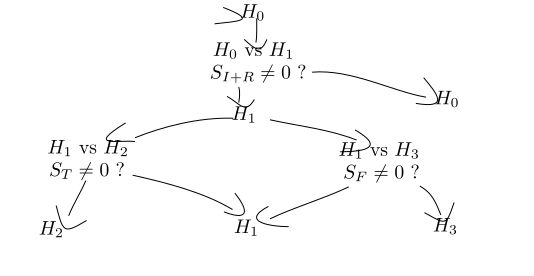
\includegraphics[width=0.7\linewidth]{./img_diagramas/estacionariedad_decidir.pdf}
%\caption{Representaci\'on diagram\'atica de la implementaci\'on en R de la prueba PSR. Se omite 
%filtrado previo mediante el algoritmo STL (ver texto).}
\label{decision_psr}
\end{figure}

\begin{figure}
\centering
\begin{lstlisting}[caption={}]
Priestley-Subba Rao stationarity Test for datos
-----------------------------------------------
Samples used              : 3072 
Samples available         : 3069 
Sampling interval         : 1 
SDF estimator             : Multitaper 
  Number of (sine) tapers : 5 
  Centered                : TRUE 
  Recentered              : FALSE 
Number of blocks          : 11 
Block size                : 279 
Number of blocks          : 11 
p-value for T             : 0.4130131 
p-value for I+R           : 0.1787949 
p-value for T+I+R         : 0.1801353 
\end{lstlisting}
\caption{Resultado mostrado tras una ejecuci\'on de la funci\'on \texttt{stationarity}. 
%El par\'ametro \texttt{n.blocks} define la cantidad grupos disjuntos para los cuales se calcular\'a 
%el estimador de la FDE.
%Cabe resaltar el antepen\'ultimo rengl\'on (\texttt{p-value for T}), seg\'un el cual se puede
%aceptar o rechazar la hip\'otesis de estacionariedad d\'ebil. 
La FDE es referida como 'Spectral Density Function' (SDF).
}
\label{res_psr}
\end{figure}

%%%%%%%%%%%%%%%%%%%%%%%%%%%%%%%%%%%%%%%%%%%%%%%%%%%%%%%%%%%%%%%%%%%%%%%%%%%%%%%%%%%%%%%%%%%%%%%%%%%
%%%%%%%%%%%%%%%%%%%%%%%%%%%%%%%%%%%%%%%%%%%%%%%%%%%%%%%%%%%%%%%%%%%%%%%%%%%%%%%%%%%%%%%%%%%%%%%%%%%
%%%%%%%%%%%%%%%%%%%%%%%%%%%%%%%%%%%%%%%%%%%%%%%%%%%%%%%%%%%%%%%%%%%%%%%%%%%%%%%%%%%%%%%%%%%%%%%%%%%
%%%%%%%%%%%%%%%%%%%%%%%%%%%%%%%%%%%%%%%%%%%%%%%%%%%%%%%%%%%%%%%%%%%%%%%%%%%%%%%%%%%%%%%%%%%%%%%%%%%
